\documentclass[11pt]{article}

% ---- packages (all standard; tectonic fetches on demand) ----
\usepackage[utf8]{inputenc}
\usepackage[T1]{fontenc}
\usepackage{lmodern}
\usepackage[margin=1in]{geometry}
\usepackage{amsmath,amssymb}
\usepackage{booktabs}
\usepackage{graphicx}
\usepackage{siunitx}
\usepackage{xcolor}
\usepackage{microtype}
\usepackage[hidelinks]{hyperref}
\usepackage{caption}
\usepackage{authblk}

\sisetup{detect-weight=true, detect-family=true}

\title{\bfseries Spatial autocorrelation makes pixel-oriented
foundation-model embeddings highly compressible:\\
per-tile vector quantization for Tessera}

\author[1]{Tessera-VQ Study}
\author[1]{S.\ Keshav}
\affil[1]{Department of Computer Science and Technology, University of Cambridge\\
\texttt{sk818@cam.ac.uk}}

\date{June 2026}

\begin{document}
\maketitle

\begin{abstract}
Geospatial foundation models now emit a dense embedding for every pixel of the
Earth's surface, trading enormous representational utility for an equally
enormous storage and serving cost. We test the hypothesis that the
\emph{spatial autocorrelation} of the landscape---the fact that, within a small
ground area, only a handful of land-cover prototypes occur---makes the
embeddings of a \emph{pixel-oriented} model far more compressible than their
raw byte count suggests, at little cost to downstream utility. We study
\textbf{Tessera}, a self-supervised model producing a 128-dimensional embedding
per ${\sim}10\,\mathrm{m}$ pixel, and compress it with \textbf{per-tile residual
vector quantization (RVQ)}: a small per-tile codebook of prototype vectors plus
a per-pixel index map. We argue, and our geometry diagnostics confirm, that this
lever is specific to pixel-oriented models: a patch-oriented model whose unit of
embedding aggregates heterogeneous sub-content produces tile-local embeddings
that are too diverse for a small codebook to capture.
We proceed in three steps. (i) \emph{Metric selection}: geometry diagnostics
(near-Gaussian but strongly anisotropic marginals; a stage-1 codebook whose
effective dimension is ${\approx}5$ against a near-full-rank residual) and a
direct sweep establish that Euclidean ($L_2$) $k$-means is the correct
quantizer, beating cosine by ${\sim}3.4\times$ on reconstruction error.
(ii) \emph{Reconstruction at scale}: over 10 large tiles ($p\in\{512,768,1024\}$,
${\sim}12\,\mathrm{km}$ windows), RVQ explains $R^2\approx0.79$ of the embedding
variance, essentially flat across the codebook split, while the byte economics
invert---at large tiles the per-tile codebook is negligible and the index map
dominates---yielding raw compression of $250$--$310\times$ over \texttt{fp32}.
(iii) \emph{Downstream validation}: on two land-cover tasks (Austrian crops,
17 classes, $8.2\mathrm{M}$ labelled pixels; Cumbrian habitats, 16 classes) under
spatial group $k$-fold, reconstructed embeddings classify
\emph{as well as raw}---if anything VQ mildly denoises them---at $p=512$, with a
small but statistically firm $8\%$ relative loss appearing only at $p=1024$.
We recommend $p=512,\,k_1=20,\,k_2=256$, stored as two byte-aligned index
planes---a gzip-coded base plane plus a raw residual plane: ${\approx}1.38$
bytes/pixel, ${\approx}93\times$ smaller than \texttt{int8} ($372\times$ over
\texttt{fp32}), with no measurable downstream accuracy loss. We further find that
a general-purpose entropy coder (gzip/\texttt{zstd}) compresses the base index
plane ${\approx}2.3\times$ better than the bespoke run-length scheme it replaces.
\end{abstract}

\section{Introduction}

Self-supervised geospatial foundation models have made it practical to attach a
learned, task-agnostic feature vector to every parcel of the Earth's surface.
\textbf{Tessera} is one such model: it produces a 128-dimensional embedding for
each ${\sim}10\,\mathrm{m}\times10\,\mathrm{m}$ pixel, capturing the local
spectral--temporal signature in a form that supports many downstream tasks
(crop typing, habitat mapping, change detection) without retraining the encoder.
The representational win comes with a storage and serving liability that scales
with the planet: stored as \texttt{int8}, a single 128-dimensional embedding is
128 bytes/pixel; as \texttt{fp32}, 512 bytes/pixel. At $10\,\mathrm{m}$
resolution a single $1024\times1024$ tile is already ${\approx}134\,\mathrm{MB}$
(\texttt{int8}); continental coverage is measured in petabytes. Compression is
therefore not a nicety but a precondition for serving these embeddings at scale.

\paragraph{Hypothesis.}
Our central claim is that this cost is largely illusory, and that the
\emph{structure of the landscape itself} provides the compression. Geographic
phenomena are spatially autocorrelated---``everything is related to everything
else, but near things are more related than distant things''
\cite{tobler1970}---and at $10\,\mathrm{m}$ resolution a single tile typically
contains only a few distinct land covers (a crop, a road, water, woodland).
If Tessera faithfully encodes ground content, then within a tile its
per-pixel embeddings should cluster tightly around a \emph{small number of
prototype vectors}. A tile of $p\times p$ pixels would then be representable by
a compact per-tile codebook of prototypes plus a per-pixel index map pointing
each pixel at its prototype---collapsing the per-pixel cost far below the raw
128 bytes, at limited cost to the embedding's downstream utility.

\paragraph{Why pixel-oriented, and not patch-oriented, models.}
This lever is not generic to foundation models; it is specific to those whose
\emph{unit of embedding is small enough that neighbouring units are near
duplicates}. Tessera is pixel-oriented: each $10\,\mathrm{m}$ pixel receives its
own vector, so spatial autocorrelation acts directly on the objects we quantize.
By contrast, a \emph{patch-oriented} model (e.g.\ a vision-transformer
masked-autoencoder that emits one token per $16\times16$ patch) embeds a unit
that already aggregates heterogeneous sub-content; adjacent patches mix different
proportions of ground cover and therefore diverge in embedding space. Within a
tile the patch embeddings span a much higher-dimensional manifold, and no
handful of prototypes captures them---a per-tile codebook either explodes in
size or reconstructs poorly. We make this contrast quantitative in
Section~\ref{sec:metric} (the stage-1 codebook of Tessera occupies an effective
dimension of ${\approx}5$, the signature of a few-prototype regime) and return to
its implications for transferability in Section~\ref{sec:discussion}. The present
study therefore uses Tessera as a case study \emph{for the pixel-oriented class},
and we are explicit that we have not measured a patch model here.

\paragraph{Contributions and structure.}
We test the hypothesis in three steps, each a section of this paper:
\begin{enumerate}
  \item \textbf{Choosing the distance metric} (Section~\ref{sec:metric}). We
  characterize the embedding geometry and show that Euclidean ($L_2$) $k$-means,
  not cosine, is the correct quantizer for this space.
  \item \textbf{Reconstruction at scale} (Section~\ref{sec:recon}). Over 10 large
  tiles we measure scale-free reconstruction fidelity and the
  \emph{compressed} byte cost, and show that the byte economics invert at large
  tiles so that the index map---not the codebook---becomes the lever.
  \item \textbf{Downstream validation} (Section~\ref{sec:downstream}). On two
  land-cover classification tasks under an honest spatial split, we show that a
  classifier trained on reconstructed embeddings matches one trained on raw.
\end{enumerate}
Joining the compressed byte cost with downstream accuracy yields a Pareto
frontier (Section~\ref{sec:pareto}) and a single engineering recommendation.

\section{Background and method}
\label{sec:method}

\paragraph{Per-tile residual vector quantization.}
Vector quantization (VQ) replaces each data vector by the nearest entry of a
learned codebook \cite{gray1984}; residual VQ (RVQ) refines this in stages, each
quantizing the residual left by the previous one \cite{jegou2011}. We apply RVQ
\emph{per tile}. For a $p\times p$ tile of embeddings, stage~1 fits a codebook of
$k_1$ coarse prototypes by $k$-means and assigns each pixel an index
$\mathrm{idx}_1\in\{0,\dots,k_1-1\}$; stage~2 fits a codebook of $k_2$ prototypes
to the stage-1 \emph{residuals} and assigns $\mathrm{idx}_2\in\{0,\dots,k_2-1\}$.
The reconstruction of a pixel is
\begin{equation}
\hat{x} \;=\; C_1[\mathrm{idx}_1] \;+\; C_2[\mathrm{idx}_2],
\end{equation}
where each codebook entry is stored as 128 \texttt{int8} values (128 bytes).
Codebooks are fit on \emph{all} finite pixels of a tile (the realistic
compression scenario), using a sampled-fit, exact-assign $k$-means with a
BLAS-GEMM distance kernel for speed.

\paragraph{Byte-cost model.}
Per pixel, the cost decomposes into a codebook term and an index term:
\begin{equation}
\underbrace{\frac{(k_1+k_2)\cdot 128}{p^2}}_{\text{codebook (amortized)}}
\;+\;
\underbrace{\vphantom{\frac{1}{1}} b(\mathrm{idx}_1) + b(\mathrm{idx}_2)}_{\text{index planes}}
\quad\text{bytes/pixel},
\label{eq:cost}
\end{equation}
where $b(\cdot)$ is the \emph{compressed} size of each index plane. The codebook
term shrinks as $1/p^2$; this single fact, developed in
Section~\ref{sec:recon}, is what makes large tiles attractive and shifts the
entire optimization onto the index planes.

\paragraph{Data and provenance.}
Embeddings are read from GeoTessera (year 2024) over ${\sim}12\,\mathrm{km}$
windows; tiles with NaN-heavy no-data edges are screened out. All numerical
results are written to Parquet with full provenance (git SHA, seed, UTC
timestamp, configuration hash); every experiment uses a fixed seed (42). The
figure and tables in this paper are generated directly from those files.

\section{Choosing the distance metric}
\label{sec:metric}

Before quantizing we characterize the embedding distribution, because its
geometry determines whether Euclidean $k$-means is appropriate and exposes the
few-prototype structure our hypothesis predicts.

\paragraph{The marginals are near-Gaussian in shape but not formally normal.}
Over 200 random one-dimensional projections, Shapiro--Wilk rejected normality
for $99\%$ of directions and Epps--Pulley for $95\%$, yet the Shapiro--Wilk
statistic sat at a median of $0.993$ (where $1.0$ is exactly Gaussian). The
rejections are the familiar large-sample artifact---millions of pixels make
negligible departures ``significant''---while the \emph{shape} is close to
Gaussian. This matters because $k$-means is the maximum-likelihood quantizer for
an isotropic Gaussian mixture; a grossly non-Gaussian space would call for a
different tool.

\paragraph{The space is strongly anisotropic.}
Per-dimension means are offset (spanning ${\approx}[-3.9,\,5.1]$; e.g.\ dimension
0 has mean ${\approx}4.2$) and per-dimension variances span a wide range
(${\approx}1.3$--$15.0$). No dimension is collapsed. Dimensions thus carry
different centres and scales, and \emph{magnitude carries signal}---a fact that
immediately disfavours any distance that discards it.

\paragraph{The codebook geometry is the hypothesis made quantitative.}
We measured the effective dimension of the two codebooks (participation ratio
and entropy effective dimension of their singular spectra). The \textbf{stage-1
(base) codebook collapses to an effective dimension of ${\approx}5$}
(participation ratio ${\approx}2.6$; $90\%$ of the energy in $7$ of $128$
directions): the per-tile base prototypes live on a low-dimensional manifold,
exactly the ``handful of land covers'' the hypothesis posits. The
\textbf{stage-2 (residual) codebook is near-full-rank} (effective dimension
${\approx}83$; participation ratio ${\approx}59$): once the few base prototypes
are removed, what remains is high-dimensional and nearly white. This two-tier
structure---a compressible base plus an incompressible residual---is the
geometric fingerprint of a pixel-oriented model under spatial autocorrelation,
and it is precisely what a patch-oriented model, lacking near-duplicate
neighbours, would not exhibit.

\paragraph{Euclidean beats cosine decisively.}
A direct sweep settles the metric. Across matched codebook sizes, the median
per-pixel reconstruction error under Euclidean $k$-means was $6.4$--$8.3$
(in embedding units), versus ${\approx}27.9$ under cosine $k$-means---a
${\sim}3.4\times$ penalty (Table~\ref{tab:metric}). Cosine discards magnitude,
which the anisotropy analysis shows is real signal here. We therefore fix
\textbf{Euclidean ($L_2$) $k$-means} as the quantizer and drop cosine from all
subsequent sweeps; because stage~1 already preserves magnitude, $L_2$ is the
meaningful metric for the residual as well.

\begin{table}[t]
\centering
\caption{Median per-pixel reconstruction error ($L_2$, embedding units) of
Euclidean vs.\ cosine $k$-means at matched codebook size $k$. Cosine $k$-means
ignores magnitude and pays a ${\sim}3.4\times$ penalty. Lower is better.}
\label{tab:metric}
\begin{tabular}{r S[table-format=2.2] S[table-format=2.2]}
\toprule
$k$ & {Euclidean $L_2$} & {Cosine} \\
\midrule
16  & 8.26 & 27.87 \\
64  & 7.18 & 27.84 \\
256 & 6.37 & {--} \\
\bottomrule
\end{tabular}
\end{table}

\section{Reconstruction at scale}
\label{sec:recon}

We next quantify how faithfully per-tile RVQ reconstructs embeddings, and at
what compressed byte cost, over a sweep of large tiles
($p\in\{512,768,1024\}$, ${\sim}12\,\mathrm{km}$ windows, $n=10$ tiles per
configuration, seed 42). To avoid the run-to-run instability of histogram-binned
error metrics, we report only \emph{scale-free} quantities: the per-pixel
relative $L_2$ error $\lVert x-\hat{x}\rVert/\lVert x\rVert$ and the coefficient
of determination $R^2 = 1 - \mathrm{Var}(x-\hat{x})/\mathrm{Var}(x)$, the
fraction of embedding variance explained.

\paragraph{Reconstruction is high and flat.}
RVQ explains $R^2\approx0.79$ of the embedding variance, and this is remarkably
\emph{flat}: across the $(k_1,k_2)$ split the spread is $\le0.004$ (about
$25\times$ smaller than the between-tile standard deviation of ${\approx}0.09$),
and across tile size it moves only from $0.798$ at $p=512$ to $0.791$ at
$p=1024$ (Table~\ref{tab:recon}). The median relative $L_2$ error rises gently
with tile size, from ${\approx}0.18$ at $p=512$ to ${\approx}0.20$ at $p=1024$
(${\sim}10\%$ worse per pixel)---a difference $R^2$, being
variance-weighted, hides, but which the downstream classifier will later feel
(Section~\ref{sec:downstream}). The flatness across the split is the key
result: \emph{fidelity does not constrain the choice of $k_1$ and $k_2$}, freeing
them to be chosen for compressibility.

\begin{table}[t]
\centering
\caption{Reconstruction fidelity over the large-tile sweep ($n=10$ tiles per
row; $R^2$ standard deviation is between-tile). $R^2$ is essentially flat across
the codebook split and across tile size; the per-pixel relative $L_2$ error
degrades mildly with $p$.}
\label{tab:recon}
\begin{tabular}{r r r S[table-format=1.3] S[table-format=1.3] S[table-format=1.3]}
\toprule
$p$ & $k_1$ & $k_2$ & {rel-$L_2$ (p50)} & {$R^2$} & {$R^2$ s.d.} \\
\midrule
512  & 64  & 1024 & 0.181 & 0.798 & 0.093 \\
512  & 256 & 256  & 0.182 & 0.796 & 0.094 \\
768  & 256 & 256  & 0.192 & 0.797 & 0.097 \\
1024 & 64  & 1024 & 0.198 & 0.791 & 0.096 \\
1024 & 256 & 256  & 0.198 & 0.791 & 0.095 \\
\bottomrule
\end{tabular}
\end{table}

\paragraph{The byte economics invert at large tiles.}
By Eq.~\eqref{eq:cost} the codebook term scales as $1/p^2$. At small tiles it
dominated the payload (90--99\% of bytes), which historically made codebook
factorization the focus. At large tiles it becomes a rounding error: at $p=512$
the codebook is only $0.13$--$0.19$ bytes/pixel, and at $p=1024$ about
$0.03$--$0.05$. The \emph{index map} now dominates, and the optimization target
shifts entirely onto compressing the two index planes---the subject of the next
section.

\section{Encoding the index map}
\label{sec:index}

Once the codebook is negligible, the compression ratio is decided almost entirely
by how the two index planes are encoded. The planes have \emph{opposite}
statistical character: the base plane rewards a good entropy coder, while the
residual plane is an irreducible floor. Extracting the most from the base plane
turns out to need a \emph{general-purpose} compressor, not the bespoke run-length
scheme that an autocorrelated map first suggests.

\paragraph{Two planes, opposite compressibility.}
The stage-1 index $\mathrm{idx}_1$ tracks land cover: neighbouring pixels share a
base prototype, so the plane is spatially smooth and rich in long runs. The
stage-2 residual index $\mathrm{idx}_2$ is, by construction, what remains after
the smooth part is removed---it is spatially white and full-rank. Any encoder must
therefore treat the planes separately, and a first design decision follows
immediately: \emph{the planes cannot be interleaved.} A 16-bit word packing
$(\mathrm{idx}_1,\mathrm{idx}_2)$ per pixel defeats compression, because the white
low byte changes at almost every pixel and breaks the structure the smooth high
byte would have offered. We therefore store two \emph{separate, byte-aligned}
planes; with $k_1,k_2\le256$ each index fits in one byte and each plane is
independently addressable and independently compressible.

\paragraph{The residual plane is an incompressible floor.}
Stored raw, $\mathrm{idx}_2$ costs exactly $1$ byte/pixel at $k_2\le256$, and this
is a hard floor: a full-rank, spatially white index at $k_2=256$ has ${\approx}8$
bits of entropy per pixel, so no lossless coder can beat one byte. Run-length
coding along a Hilbert scan in fact \emph{inflates} it to $1.31$--$1.62$
bytes/pixel (Table~\ref{tab:index2})---the run headers cost more than the absent
runs save. This is also why $k_2=256$ is the right operating point: it spends the
full byte to maximize residual codewords (and hence fidelity headroom) at no extra
cost, whereas $k_2=512$ or $1024$ would push the dominant plane past a byte and
double it for negligible $R^2$ gain.

\paragraph{Coding the base plane: a general-purpose coder beats run-length encoding.}
The base plane is smooth, which makes byte-aligned run-length encoding (RLE) the
obvious first choice---and the one used in our initial sweep. But RLE captures only
\emph{immediate} repetition (a run of identical neighbours) and entropy-codes
nothing, whereas the base indices are both repetitive at \emph{longer} range and
far from uniformly distributed (a few prototypes dominate each tile). A
general-purpose coder exploits both. Measured on real base-index maps from four
contrasting biomes (Amazon forest, Sahel, Welsh pasture, Iowa cropland;
Table~\ref{tab:index}), \textbf{gzip (DEFLATE) is $2.1$--$2.6\times$ smaller than
byte-aligned RLE in every cell}, and \texttt{zstd} a few percent smaller still. At
$p=512,\,k_1=20$ the base plane falls from $0.63$ bytes/pixel under RLE to $0.24$
under gzip ($0.22$ under \texttt{zstd}). Tellingly, gzip applied \emph{after} RLE
($0.27$ bytes/pixel) is \emph{worse} than gzip on the raw plane: RLE has already
discarded the symbol-frequency structure that DEFLATE's Huffman stage would
exploit. We therefore drop RLE in favour of a stock entropy coder---gzip for
universality, \texttt{zstd} for a marginal further gain---on the raw byte plane.

\paragraph{Scan order barely matters.}
One might expect a space-filling curve (Morton or Hilbert) to help by improving
2-D locality before coding. It does not, for either coder. Among RLE orderings the
plain raster scan is already best (row $\le$ Hilbert $<$ Morton), and for gzip the
scan changes the result by under $3\%$. The reason is the shape of real land cover
at this scale: fields and parcels are elongated and roughly axis-aligned, so a
raster scan already runs \emph{along} their boundaries, whereas a curve's recursive
zig-zag repeatedly crosses them. The practical consequence is welcome---no
space-filling machinery is needed; the plain row-major byte plane fed to
gzip/\texttt{zstd} is both the simplest and the best encoder.

\paragraph{Smaller $k_1$ compresses better.}
The base-plane cost falls \emph{monotonically} as $k_1$ shrinks under every coder
(Table~\ref{tab:index}): under gzip, from $0.44$ bytes/pixel at $k_1=128$ to
$0.24$ at $k_1=20$ ($p=512$). Fewer base prototypes give a coarser, smoother, more
predictable map. Since Section~\ref{sec:recon} showed fidelity is flat across
$k_1$ and Section~\ref{sec:downstream} will show downstream $F_1$ is too, $k_1$ is
free to be chosen purely for compressibility---and smallest is best. This makes
precise the practitioner observation that ``$k_1\approx20$ already captures the
landscape''.

\begin{table}[t]
\centering
\caption{Base-plane ($\mathrm{idx}_1$) cost in bytes/pixel under byte-aligned RLE,
gzip (DEFLATE), and \texttt{zstd}, with the incompressible residual floor and
amortized codebook, at $k_2=256$. Means over four large tiles from contrasting
biomes (seed 42); the RLE column reproduces the 10-tile sweep (e.g.\ $0.627$
vs.\ $0.632$ at $p=512,\,k_1=20$). gzip is $2.1$--$2.6\times$ smaller than RLE
everywhere; \texttt{total} and ``$\times$\,\texttt{int8}'' use gzip.}
\label{tab:index}
\begin{tabular}{r r S[table-format=1.3] S[table-format=1.3] S[table-format=1.3] S[table-format=1.1] S[table-format=1.3] S[table-format=1.3] S[table-format=3.1]}
\toprule
$p$ & $k_1$ & {RLE} & {gzip} & {zstd} & {idx2} & {codebook} & {total} & {$\times$\,\texttt{int8}} \\
\midrule
512  & 20  & 0.627 & 0.240 & 0.219 & 1.0 & 0.135 & 1.375 & 93.1 \\
512  & 32  & 0.735 & 0.296 & 0.272 & 1.0 & 0.141 & 1.437 & 89.1 \\
512  & 128 & 0.942 & 0.444 & 0.415 & 1.0 & 0.188 & 1.632 & 78.4 \\
1024 & 20  & 0.593 & 0.235 & 0.212 & 1.0 & 0.034 & 1.269 & 100.9 \\
1024 & 128 & 0.955 & 0.458 & 0.420 & 1.0 & 0.047 & 1.505 & 85.0 \\
\bottomrule
\end{tabular}
\end{table}

\begin{table}[t]
\centering
\caption{The residual plane does not compress. Run-length coding along a Hilbert
scan of $\mathrm{idx}_2$ \emph{inflates} it past its raw $1$ byte/pixel,
confirming that $\mathrm{idx}_2$ is spatially white and setting the
incompressible floor ($k_2=256$).}
\label{tab:index2}
\begin{tabular}{r r S[table-format=1.1] S[table-format=1.2]}
\toprule
$p$ & $k_1$ & {idx2 raw} & {idx2 Hilbert+RLE} \\
\midrule
512  & 20  & 1.0 & 1.38 \\
512  & 128 & 1.0 & 1.62 \\
1024 & 20  & 1.0 & 1.31 \\
1024 & 128 & 1.0 & 1.56 \\
\bottomrule
\end{tabular}
\end{table}

Combining the two planes and the codebook, per-tile RVQ achieves
$310$--$400\times$ compression over \texttt{fp32} ($78$--$101\times$ over
\texttt{int8}; Table~\ref{tab:index}) \emph{before} we have spent any
downstream-accuracy budget. Whether that budget is in fact zero is the question
the next section settles.

\section{Downstream validation}
\label{sec:downstream}

Reconstruction error is a proxy. What ultimately matters for a foundation-model
product is whether a classifier trained on \emph{reconstructed} embeddings
performs as well as one trained on \emph{raw}. We test this on two labelled
land-cover datasets, under a protocol designed to avoid the most common way such
comparisons are inflated.

\paragraph{Tasks.}
\textbf{Austria}: 17 crop classes (heavily imbalanced) over $8.2\mathrm{M}$
labelled pixels---enough scale for tight error bars. \textbf{Cumbria/Naddle}: 16
UK habitat classes over a much smaller labelled extent (${\approx}1.1\times10^5$
pixels)---useful as a second domain but statistically noisy. For each tile we
fetch raw embeddings, fit per-tile RVQ, reconstruct, rasterize the labels, and
extract labelled pixels from the \emph{raw} and \emph{reconstructed} rasters,
yielding paired feature sets with identical labels.

\paragraph{Protocol: spatial group $k$-fold.}
We train the same Random Forest \cite{breiman2001} on raw vs.\ reconstructed
features under \textbf{4-fold spatial group cross-validation}, holding out whole
tiles per fold. This is essential: a random pixel-level $k$-fold places
spatially adjacent (hence autocorrelated) pixels in both train and test,
inflating absolute accuracy and---worse for our purpose---\emph{flattering VQ},
because a near-duplicate of every test pixel sits in training. Holding out whole
tiles removes that leak. The metric is the per-configuration difference
$\Delta F_1 = F_1(\text{raw}) - F_1(\text{recon})$ in macro-$F_1$; positive
$\Delta F_1$ is a loss from compression. Absolute macro-$F_1$ is low
($\approx0.20$--$0.22$) because spatial hold-out over many fine-grained classes
is genuinely hard; the valid signal is the \emph{relative} raw-vs-recon
comparison under an identical protocol, not the absolute ceiling.

\paragraph{Result: $p=512$ is downstream-lossless.}
At $p=512$, $\Delta F_1\approx0$ at every $k_1$ ($|\Delta/\sigma|<1$), and
retention (recon\,/\,raw $F_1$) is consistently $\ge1.0$: reconstructed
embeddings classify \emph{at least as well} as raw, and often marginally better,
consistent with VQ mildly denoising the embeddings. At the recommended
$k_1=20$, raw $F_1=0.204$ vs.\ recon $F_1=0.211$ on Austria
(Table~\ref{tab:downstream}).

\paragraph{Result: $p=1024$ carries a small but firm loss.}
At $p=1024$, Austria shows $\Delta F_1\approx+0.017$ ($\approx8\%$ relative) at
$\Delta/\sigma\approx6$--$7.5$. With a between-fold standard deviation of
${\approx}0.002$ over $8.2\mathrm{M}$ pixels this is not noise: a single codebook
covering ${\approx}10^6$ pixels is coarser per pixel than four codebooks each
covering $512^2$, the per-pixel penalty that the variance-weighted $R^2$ hid but
the classifier feels. Cumbria, with its $4$-tile scale and large variance
(s.d.\ up to ${\approx}0.06$), cannot resolve a difference this small and is
consistent with both zero and the Austria effect. Within a tile size, $k_1$ does
not affect $F_1$, so $k_1$ is free to be chosen for compressibility.

\begin{table}[t]
\centering
\caption{Downstream macro-$F_1$ (Austria, 17 classes, $8.2\mathrm{M}$ pixels,
4-fold spatial group CV) for raw vs.\ reconstructed embeddings. $\Delta F_1>0$ is
a loss. $p=512$ is lossless (recon $\ge$ raw); $p=1024$ shows a firm
${\approx}8\%$ relative loss ($\Delta/\sigma\approx7.5$ at $k_1=20$).}
\label{tab:downstream}
\begin{tabular}{r r S[table-format=1.3] S[table-format=1.3] S[table-format=2.3] S[table-format=1.3]}
\toprule
$p$ & $k_1$ & {$F_1$ raw} & {$F_1$ recon} & {$\Delta F_1$} & {s.d.} \\
\midrule
512  & 20  & 0.204 & 0.211 & -0.007 & 0.009 \\
512  & 32  & 0.204 & 0.205 & -0.000 & 0.011 \\
512  & 128 & 0.204 & 0.210 & -0.006 & 0.006 \\
1024 & 20  & 0.204 & 0.188 &  0.017 & 0.002 \\
1024 & 32  & 0.204 & 0.184 &  0.020 & 0.003 \\
1024 & 128 & 0.204 & 0.193 &  0.011 & 0.008 \\
\bottomrule
\end{tabular}
\end{table}

\paragraph{Reconstruction proxy vs.\ downstream truth.}
The two metrics \emph{agreed on the split} (both flat across $k_1$,$k_2$) but
\emph{disagreed on $p$}: $R^2$ called $p=512$ and $p=1024$ equivalent, while the
classifier did not. Intrinsic reconstruction error is thus necessary but not
sufficient, and the downstream task must remain the arbiter for any choice that
$R^2$ reports as a tie.

\section{The Pareto frontier and recommendation}
\label{sec:pareto}

Joining the compressed byte cost (Section~\ref{sec:index}) with downstream
retention (Section~\ref{sec:downstream}) gives the frontier in
Figure~\ref{fig:pareto}. Only two points are non-dominated, both at $k_1=20$
(Table~\ref{tab:pareto}): $p=512$ at $1.38$ bytes/pixel and downstream-lossless,
and $p=1024$ at $1.27$ bytes/pixel but with the significant $8\%$ relative loss.
The frontier's membership is encoder-invariant---within a tile size, smaller
$k_1$ shrinks the base plane under every coder while leaving $F_1$ flat---so
switching the base-plane coder from RLE to gzip rescales the compression axis
(raising all ratios) without changing which configurations are non-dominated.

\begin{table}[t]
\centering
\caption{The two non-dominated configurations, with the base plane gzip-coded.
$p=1024$ buys ${\approx}8\%$ more compression for ${\approx}8\%$ relative
accuracy---a poor trade for a product whose value \emph{is} the embedding's
downstream utility.}
\label{tab:pareto}
\begin{tabular}{l S[table-format=1.2] S[table-format=3.0] S[table-format=3.0] l}
\toprule
configuration & {bytes/px} & {$\times$\,\texttt{int8}} & {$\times$\,\texttt{fp32}} & downstream \\
\midrule
\textbf{$p=512,\,k_1=20,\,k_2=256$} & 1.38 & 93 & 372 & lossless ($\Delta F_1\approx0$) \\
$p=1024,\,k_1=20,\,k_2=256$         & 1.27 & 101 & 403 & $-8\%$ relative $F_1$ (significant) \\
\bottomrule
\end{tabular}
\end{table}

\begin{figure}[t]
\centering
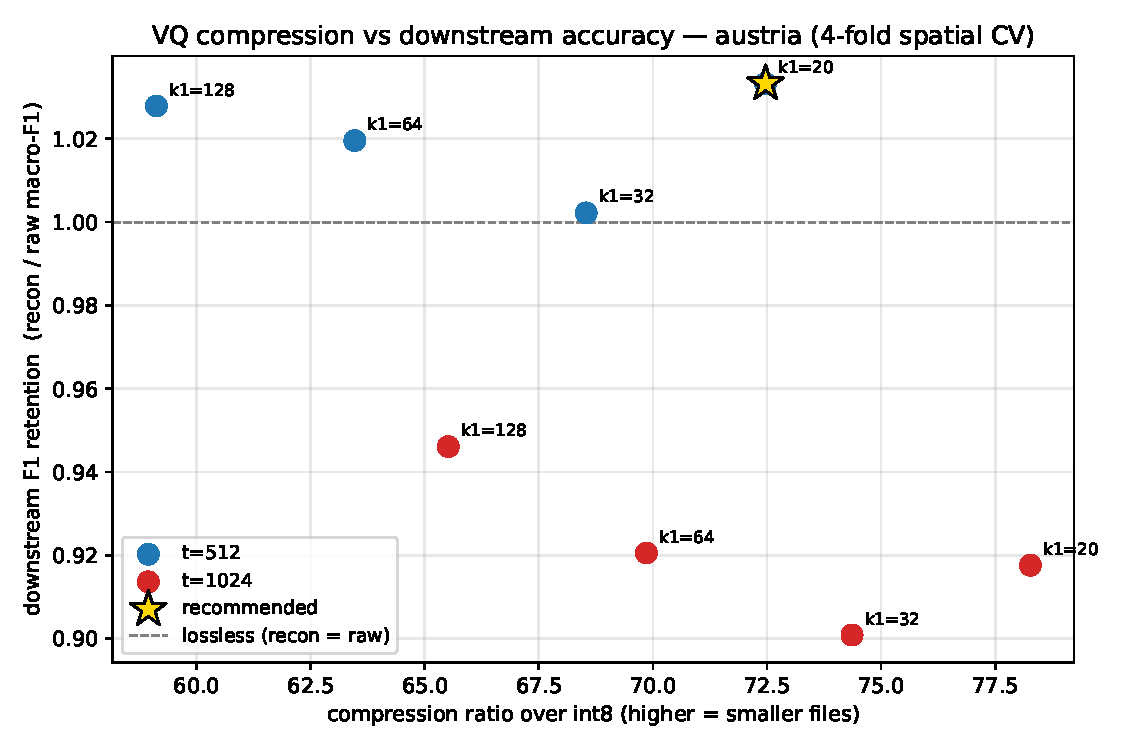
\includegraphics[width=0.85\linewidth]{../figures/phase4_pareto.pdf}
\caption{Downstream $F_1$ retention (recon\,/\,raw macro-$F_1$, Austria, 4-fold
spatial CV) against compression ratio over \texttt{int8}, with the base index
plane gzip-coded (Section~\ref{sec:index}). The recommended configuration
($p=512,\,k_1=20$, star) sits above the lossless line at ${\approx}93\times$; the
$p=1024$ points trade ${\approx}8\%$ accuracy for modest extra compression. The
non-dominated set ($k_1=20$ at each tile size) is encoder-invariant. Here $p$
denotes the tile size in pixels.}
\label{fig:pareto}
\end{figure}

\paragraph{Recommendation.}
We recommend \textbf{$p=512,\,k_1=20,\,k_2=256$}. Per $512\times512$ serving
tile, store: \texttt{codebook1} ($20\times128$ \texttt{int8}) and
\texttt{codebook2} ($256\times128$ \texttt{int8}), amortizing to
${\approx}0.14$ bytes/pixel; an \texttt{idx1} plane (values $0$--$19$), stored as
a raw row-major byte plane and \textbf{gzip-compressed} (DEFLATE),
${\approx}0.24$ bytes/pixel (\texttt{zstd} reaches ${\approx}0.22$); and an
\texttt{idx2} plane (values $0$--$255$), raw at $1$ byte/pixel. The total is
${\approx}1.38$ bytes/pixel, ${\approx}93\times$ smaller than \texttt{int8}-served
embeddings ($372\times$ over \texttt{fp32}), reconstructable to within
downstream-classifier tolerance. The alternative $p=1024$ aligns with the native
GeoTessera UTM tile---an integration convenience---and is the right choice
\emph{only} if that alignment is judged worth the $8\%$ accuracy cost; it was not
here.

\section{Discussion}
\label{sec:discussion}

\paragraph{The hypothesis holds, for pixel-oriented models.}
The chain of evidence supports the central claim. The stage-1 codebook's
${\approx}5$-dimensional effective rank shows that, within a tile, Tessera's
per-pixel embeddings really do cluster around a handful of prototypes; the
inverted byte economics show that this structure delivers two orders of magnitude
of compression at large tiles; and the downstream tasks show that the
reconstruction is faithful enough to be \emph{free} of accuracy cost at $p=512$.
Spatial autocorrelation is doing the work exactly as posited.

\paragraph{Why this should not transfer to patch-oriented models.}
The mechanism depends on near-duplicate neighbours. A patch-oriented model
embeds a unit that already integrates over heterogeneous sub-content, so adjacent
units diverge and the within-tile manifold is high-dimensional---the analogue of
our stage-1 codebook would not collapse to ${\approx}5$ dimensions, and a small
per-tile codebook would either reconstruct poorly or grow until it forfeits the
compression. We did not measure a patch model and so state this as a falsifiable
prediction rather than a result: a per-tile-codebook effective-rank diagnostic
(Section~\ref{sec:metric}) applied to a patch model's tile-local embeddings would
test it directly, and is the natural next experiment.

\subsection*{Deployment options}
\label{sec:deploy}

A result that compression is downstream-free is only useful if it can be
delivered. Two architectures are available (Figure~\ref{fig:deploy}), and they
differ in where the quantization happens and who pays for it.

\paragraph{Bolt-on VQ.}
The first option leaves Tessera unchanged and adds VQ as a \emph{bolt-on}: a
service that fetches raw embeddings and quantizes them on demand. This is the
already-deployed path---a local service co-located with the Tessera Embeddings
Explorer (TEE)---and it has two independent design axes. The first is the
\emph{source} of the raw embeddings: a local Cambridge store, or object storage
in S3. The second is the \emph{access scope}: serving only TEE users, or opening
the fast path to anyone. The two axes carry the central engineering tension.
Restricting access to TEE keeps the compute bounded but limits the benefit to a
single application; opening it broadens the benefit but, because the bolt-on
quantizes \emph{on demand} (a per-tile $k$-means fit per request), heavy public
use concentrates a substantial CPU load on the host. Source and access also
interact: serving embeddings drawn from S3 to a wide audience requires the
bolt-on to have low-latency S3 access, or the fetch dominates the response.

\paragraph{A staged rollout.}
These axes suggest a natural progression that defers cost until demand justifies
it (Figure~\ref{fig:deploy}). \emph{Stage 1}---TEE-only access, embeddings from
the Cambridge store---is the current state: lowest compute, narrowest reach, and
the simplest thing that delivers the saving to one application. \emph{Stage 2}
keeps access TEE-only but widens the source to Cambridge \emph{or} S3, which
requires giving the bolt-on fast S3 access but lets it serve regions not held
locally. \emph{Stage 3} opens the fast path to anyone; the on-demand compute then
has to be met by a large provisioned server, the first point at which serving
cost becomes a first-order concern.

\paragraph{Native VQ, and why our result enables it.}
The fourth option abandons the bolt-on entirely and folds VQ into Tessera's
\emph{embedding-generation} pipeline, releasing embeddings in VQ format as the
\emph{only} distributed form. This removes per-request quantization compute
outright and pushes the ${\approx}93\times$/$372\times$ saving back to the storage layer,
where it reduces the footprint of the whole archive rather than of one serving
path. Its precondition is exactly the question this paper answers: one can
release VQ-only embeddings only if they are \emph{good enough} for downstream use.
Our finding that $p=512$ reconstruction is downstream-lossless
(Section~\ref{sec:downstream}) is what makes Stage~4 defensible rather than
speculative---and it is why the staged path loops back to a native integration
once the fidelity evidence is in hand.

\begin{figure}[t]
\centering
\includegraphics[width=0.62\linewidth]{../figures/deployment_options.pdf}
\caption{Deployment options for VQ. The bolt-on (blue) quantizes on demand atop
raw embeddings and is governed by two axes---embedding source (Cambridge vs.\ S3)
and access scope (TEE-only vs.\ open). A staged rollout widens source, then
access, before---if reconstruction fidelity suffices---dispensing with the
bolt-on for a native integration (green) that releases embeddings in VQ format
only, moving the saving to the storage layer.}
\label{fig:deploy}
\end{figure}

\paragraph{Limitations.}
(i) Absolute downstream $F_1$ is low (${\approx}0.20$) under spatial hold-out on
fine-grained classes; our conclusion rests on \emph{relative} retention, the
correct quantity for a compression study, but we have not characterized absolute
task ceilings. (ii) We used two datasets, one classifier (Random Forest), and
pixel-only features; spatial-context classifiers or other tasks could be more
sensitive to the lost residual and warrant a check before broad deployment.
(iii) The reconstruction sweep used 10 large tiles; while the between-tile
variance is reported and the downstream experiments are at much larger scale, a
wider reconstruction sweep would tighten the fidelity estimates. (iv) $k_1$ was
swept on $\{20,32,64,128\}$; $k_1<20$ may compress \texttt{idx1} further at
still-zero $F_1$ cost and is worth probing.

\section{Conclusion}

We tested, and confirmed, the hypothesis that spatial autocorrelation renders
pixel-oriented foundation-model embeddings highly compressible at little cost to
fidelity, using Tessera as a case study. Choosing the distance metric first
($L_2$, justified by the embedding geometry), then measuring reconstruction at
scale, then validating on two downstream land-cover tasks, we find that per-tile
residual VQ at $p=512,\,k_1=20,\,k_2=256$---with a gzip-coded base index plane---
compresses Tessera embeddings by ${\approx}93\times$ over \texttt{int8}
($372\times$ over \texttt{fp32}) with no measurable downstream accuracy loss. The
compression is a direct consequence of the
landscape's structure, and---we predict---specific to models whose unit of
embedding is small enough for that structure to act on.

\paragraph{Reproducibility.}
All results derive from versioned Parquet outputs with git SHA, seed, UTC
timestamp, and configuration hash:
\texttt{phase3/large\_v1\_large\_recon.parquet} ($R^2$, relative $L_2$);
\texttt{phase3/idx\_v2\_index\_compression.parquet} (compressed bytes/pixel);
\texttt{phase4/\{austria,cumbria\}\_downstream.parquet} (downstream $F_1$). The
Pareto figure is generated by \texttt{scripts/phase4\_pareto.py}; the
RLE-vs-gzip/\texttt{zstd} base-plane comparison (Table~\ref{tab:index}) by
\texttt{scripts/phase3\_gzip\_vs\_rle.py} (four-biome diagnostic, seed 42; pending
promotion to a provenance-tagged Parquet over the full bbox set).

\begin{thebibliography}{9}
\bibitem{tobler1970} W.~R.\ Tobler. A computer movie simulating urban growth in
the Detroit region. \emph{Economic Geography}, 46:234--240, 1970.
\bibitem{gray1984} R.~M.\ Gray. Vector quantization. \emph{IEEE ASSP Magazine},
1(2):4--29, 1984.
\bibitem{jegou2011} H.~J\'egou, M.\ Douze, and C.\ Schmid. Product quantization
for nearest neighbor search. \emph{IEEE TPAMI}, 33(1):117--128, 2011.
\bibitem{breiman2001} L.\ Breiman. Random forests. \emph{Machine Learning},
45(1):5--32, 2001.
% TODO: add the Tessera model reference and the Robinson \& Corley compression
% frontier reference once citation details are confirmed.
\end{thebibliography}

\end{document}
